\documentclass[a4paper,12pt]{article}
\usepackage[margin=1in]{geometry}

\usepackage[T2A]{fontenc}			% кодировка
\usepackage[utf8]{inputenc}			% кодировка исходного текста
\usepackage[english,russian]{babel}	% локализация и переносы
\usepackage{graphicx}                % Математика
\usepackage{amsmath,amsfonts,amssymb,amsthm,mathtools} 
\usepackage{mathtext}
\usepackage[T2A]{fontenc}
\usepackage[utf8]{inputenc}

\usepackage{wasysym}

%Заговолок
\author{Бичина Марина 
группа Б04-005 1 курса ФЭФМ}
\title{}
\date{}


\begin{document} % начало документа

\begin{center}
\begin{Large}
{Бичина Марина Б04-005, Лабораторная работа №. 5.10.1 <<Электронный парамагнитный резонанс>>}
\end{Large}
\end{center}
\paragraph{Цель работы:} 
\begin{enumerate}
\itemsep0em
\item Исследовать электронный парамагнитный резонанс в молекуле ДФПГ
\item определить g-фактор электрона
\item измерить ширину линии электронного парамагнитного резонанса (ЭПР)
\end{enumerate}

\paragraph{Теоретическая справка:}
\paragraph{}
В методе ЭПР изучается резонансное поглощение переменного электромагнитного поля в образце в зависимости от контролируемых экспериментатором внешних условий: постоянного магнитного поля, частоты колебаний переменного поля, температуры и т.д. \\
Простейшей моделью для рассмотрения ЭПР является система из невзаимодействующих
частиц со спином $S = 1/2$, помещённая во внешнее магнитное поле. В отсутствие
магнитного поля энергии состояний с проекцией спина $S_Z = \pm 1/2$ совпадают. Из-за эффекта Зеемана энергии состояний с различными проекциями спина начинают различаться. Если направить на нашу систему поток излучения с энергией, равной разнице энергий этих состояний 
\begin{equation}\label{2}
h \nu = g\mu_B B,
\end{equation} 
то станут возможны индуцированные переходы между состояниями. Эти переходы происходят с поглощением или испусканием фотона в зависимости от того, в каком из состояний была система до взаимодействия с излучением. В отличие от оптических переходов между электронными уровнями энергии в атоме, типичная частота переменного поля в ЭПР эксперименте составляет порядка 10 ГГц (а в нашем лабораторном эксперименте около 100 МГц), что соответствует энергии фотона менее 1К. Поэтому, за исключением очень низких температур, заселённость обоих спиновых подуровней с $S_Z = \pm 1/2$ близка. \\
В «классическом» подходе рассматривается прецессия магнитного момента во внешнем поле при отклонении магнитного момента от равновесия. Классический магнитный диполь стремится выровняться вдоль силовых линий магнитного поля, при отклонении от равновесия возникает возвращающий механический момент $\mathbf{T} = \mathbf{M}\times \mathbf{B}$. Так как магнитный и механический момент иона связаны друг с другом гиромагнитным отношением $\gamma$ как $\mathbf{M}=\gamma \mathbf{J}$ , где $\mathbf{J}$ - это полный момент импульса, то с учётом уравнения динамики
$\frac{d}{dt}\mathbf{J} = \mathbf{T}$, получим уравнение прецессии магнитного момента
\[\dfrac{d}{dt}\mathbf{M} = \gamma \mathbf{M} \times \mathbf{B}.\] 
Аналогично
с известной задачей о прецессии гироскопа можно заметить, что при отклонении магнитного момента от направления магнитного поля возникает незатухающая прецессия вокруг направления поля с угловой скоростью $\boldsymbol{\Omega} = -\gamma \mathbf{B}$, частота этой прецессии $\Omega_L = \gamma B$ называется ларморовской. При совпадении частоты переменного поля, перпендикулярного основному, с ларморовской частотой возможно возникновение резонансного поглощения.

\paragraph{Описание установки:}
\paragraph{}
Образец (порошок ДФПГ) в стеклянной ампуле помещяется внутрь катушки индуктивнсоти, входящей в состав колебательного контура. Конденсатор, входящий в состав колебательного контура, состоит из двух пластин, разделенных воздушным зазором, одна из пластин может перемещаться поворотом штока. \\ Колебания в контуре возбуждаются антенной, соединённой с генератором частоты (ВЧ) Г4-116. Амплитуда колебаний поля в катушке индуктивности измеряется по наводимой в петле связи ЭДС индукции. Высокочастотные колебания ЭДС индукции в приёмном контуре детектируются диодом, измеряемая при помощи осциллографа низкочастотная огибающая этого сигнала пропорциональна квадрату амплитуды колебаний поля в катушке.
	\begin{figure}[h!]
	    \centering
			\caption{Схема установки.}
			\label{fig:equip}
			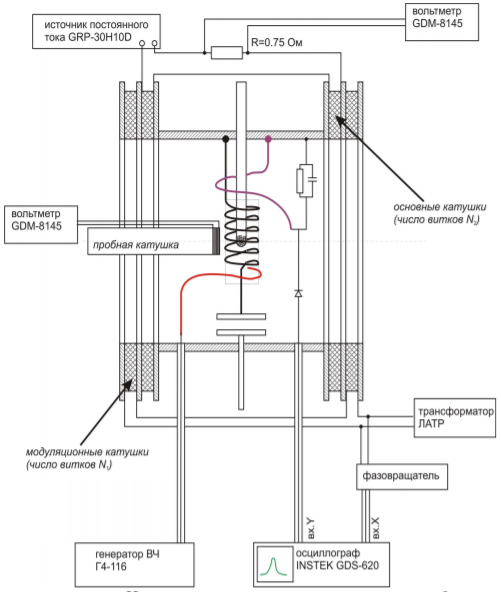
\includegraphics[scale=0.7]{setup.png}
	\end{figure}
	
	Постоянное магнитное поле создаётся пропусканием тока от источника постоянного тока через основные катушки. При этом при помощи вольтметра измеряется падение напряжения на резисторе в цепи основных катушек. Переменное поле небольшой амплитуды создаётся подачей на модуляционные катушки напряжения с регулируемого трансформатора ЛАТР. Для измерения амплитуды колебаний переменного поля используется пробная катушка известной геометрии, подключенная к вольтметру.
	
\newpage
\paragraph{Ход работы:}
\begin{enumerate}
\itemsep0em
\item  Запишем параметры катушек в  Таблицу \ref{table:coils}:
	    
	    \begin{table}[h]
	    \label{table:coils}
	    \centering
            \begin{tabular}{|l|l|l|}
            \hline
            \textbf{Катушка} & $N$ & $D$, см \\ \hline \hline
            Основная         & 6700         & $25\pm1$             \\ \hline
            Модуляционная    & 5000         & $30\pm1$             \\ \hline
            Пробная          & 45           & $1.52\pm0.01$             \\ \hline
            \end{tabular}
            \caption{Параметры катушек.}
        \end{table}
\item 
		Настроим генератор на частоту колебательного конутра. Получаем резонансную частоту:
		\begin{equation*}
			\nu = (160 \pm 1) \ \text{Мгц}.			
		\end{equation*}
		Запишем значение напряжения на резисторе в цепи основных катушек:
		\begin{equation*}
					\varepsilon_1
 = (137 \pm 1) \ \text{мВ}.
		\end{equation*}
\item Определим ширину линии ЭПР (полуширина на на полувысоте линии резонасного поглощения):
		\begin{equation*}
			\Delta B = \frac{A_{1/2}}{A_{\text{полн}}}B_\text{мод},
		\end{equation*}
		где $A_\text{полн}$ -- полный размах модулирующего поля, \\$A_{1/2}$ -- ширина кривой на полувысоте,\\ $B_\text{мод}$ -- амплитуда модулирующего поля.
		\begin{equation*}
			\begin{gathered}
				A_\text{полн} = (6 \pm 0.2 ) \ \text{дел}, \ A_{1/2} = (\frac{4}{5} \pm 0.2) \ \text{дел} \\
				B_\text{мод} = \sqrt{2} \frac{2\varepsilon}{\pi^2d^2N_{\text{проб}}\nu_{\text{мод}}} = 21\pm 5\;\; \text{Гс},
			\end{gathered}
		\end{equation*}
		где $\varepsilon = 3.85$ мВ -- ЭДС индукции при внесении пробной катушки,\\ $N_{\text{проб}}$ -- число витков катушки,\\ $d$ -- диаметр катушки,\\ $\nu_{\text{мод}}$ -- частота модулирующего напряжения (50 Гц).\\
		Погрешность была посчитана по формуле
\[\sigma_{B_{\text{мод}}}=\sqrt{\left(\dfrac{\partial B_{\text{мод}}}{\partial \mathcal{E}} \right)^2 \sigma^2_\mathcal{E} + \left(\dfrac{\partial B_{\text{мод}}}{\partial d} \right)^2 \sigma^2_{d}},\]

		
Получим:
$$\Delta B =(2.8\pm 0.2)\;\;\text{Гс}$$
	Где погрешность посчитана как 	
	\[\sigma_{\Delta B} = \sqrt{ \left(\dfrac{\partial \Delta B}{\partial A_{\text{полн}}} \right)^2 \sigma^2_{A_{\text{полн}}} +  \left(\dfrac{\partial \Delta B}{\partial A_{\text{1/2}}} \right)^2 \sigma^2_{A_{\text{1/2}}} + \left(\dfrac{\partial \Delta B}{\partial B_{\text{мод}}} \right)^2 \sigma^2_{B_{\text{мод}}} }.\]
	\item Рассчитав поле, создаваемое основными катушками,
		
		\begin{equation*}
		    B_0 = \frac{4 k\varepsilon_1}{2\pi\nu_{\text{мод}} N \pi d^2} = (76 \pm 1) \;\;\text{Гс}.
		\end{equation*}
		
		Найдем $g$-фактор электрона:
		
		\begin{equation*}
			g = \frac{h\nu}{\mu_BB_0} = \frac{6.63\cdot 10^{-27}\cdot 160\cdot 10^{6}}{927.4\cdot 10^{-23}\cdot 76} = 1.5 \pm 0.3
		\end{equation*}
погрешность считалась по формуле
\[\sigma_g = \sqrt{ \left( \dfrac{\partial g}{\partial \nu}\right)^2 \sigma_{\nu}^2 + \left( \dfrac{\partial g}{\partial B_0}\right)^2 \sigma_{B_0}^2}.\]		
\end{enumerate}
\paragraph{Выводы:}
\begin{enumerate}
\item Мы исследовали электронный парамагнитный резонанс в молекуле ДФПГ
\item Нашли ширину линий ЭПР $\Delta B = 2.8 \pm 0.2~\text{Гс}$.
\item Определили g-фактор электрона, равный $g = 1.5 \pm 0.3$ (для сравнения, табличным для электрона является значение g = 2,0023), что является весьма точным результатом для нашего метода исследования
\end{enumerate}
\end{document}